Epidemic outbreaks include a spectrum of illness, including
asymptomatic cases that can be mild and/or subclinical.
As such, symptomatic cases are the predominant focus of treatment and usually represent
the bulk of reported cases. However, infected individuals who are asymptomatic
yet infectious can be a critical, albeit poorly characterized
factor in the spread of pathogens, as well as 
present challenges for control.
Asymptomatic individuals
are hard to trace, unlikely to self-isolate,
may move outside of quarantine,  
retain normal social and travel patterns, and potentially spark new
outbreaks.
The COVID-19 outbreak has raised significant
questions regarding the role of asymptomatic cases~\citep{fauci_nejm2020}.
%For example, the incidence of asymptomatic
%infection was estimated to be
%approximately 33\% (or higher) 
%from an outbreak of COVID-19 on the Princess Cruises ship~\citep{mizumoto_2020}.
A key focus has been on estimating asymptomatic prevalence (see~\citep{mizumoto_2020}), e.g., what fraction of individuals have asymptomatic infections relative to those with symptomatic infections?
%.(i) What fraction of newly infected individuals
%have mild and/or subclinical infections rather than severe and/or
%clinical infections? (ii) What is the time-scale over which 
%individuals who have mild and/or subclinical cases remain
%infectious? (iii) How infectious are individuals
%with mild and/or subclinical infections relative to those
%with severe symptoms?  
Here, we attempt to address the impact of asymptomatic cases differently, by relating 
individual-level features of asymptomatic cases (e.g., the probability
of initiating an asymptomatic case, asymptomatic case duration, and
the tranmission rates from asymptomatic individuals) to dynamics at the
population scale. That is, rather than focusing on the prevalence
of asymptomatic cases, we are interested in understanding the
relevance of asymptomatic infections to secondary case production -- including
to the production of symptomatic cases.
%Our purpose is to characterize key drivers of contribution to
%secondary cases during an outbreak by `asymptomatic' individuals --
%and help characterize the relevance of asymptomatic transmission to
%outbreak dynamics and control.

To begin, consider a renewal equation variant in which incidence $i$ is divided into two categories -- $i_a$ and $i_s$ -- corresponding to incidence of asymptomatic and symptomatic cases, respectively. 
Both types of individuals can infect others, but, they differ in their intrinsic reproduction numbers, ${\cal{R}}_a$ and ${\cal{R}}_s$, as well as intrinsic generation-interval distributions, $g_a(\tau)$ and $g_s(\tau)$, reflecting their differences in the abilities to transmit and the courses of infection.
Generation intervals, which are defined as the time between when an individual is infected and when that individual infects another person, depend on the natural history of infection:
an individual with subclinical, and fast-clearing, symptoms is likely to have short generation intervals, whereas an individual with mild, but long-lasting, symptoms is likely to have long generation intervals.
In total, the dynamics of susceptibles and incidence are:
\begin{eqnarray}
\dot{S}&=&-i(t) \\
i(t)&=&\mathcal R_a S \int_0^\infty i_a(t-\tau) g_a(\tau) \mathrm{d}\tau + \mathcal R_s S \int_0^\infty i_s(t-\tau) g_s(\tau) \mathrm{d}\tau.
\end{eqnarray}
Here, $p$ is the fraction of asymptomatic cases that are generated for each infected individual ($i_a(t)= p i(t)$), and $1-p$ is the fraction of symptomatic cases that are generated for each infected individual ($i_s(t)= (1-p) i(t)$).

%To begin, consider a SEIR model variant in which there are two infectious categories --
%$I_a$ and $I_s$ -- corresponding to asymptomatic and symptomatic cases,
%respectively. Both types of individuals can infect others, but,
%only symptomatic cases can lead to fatalities, denoted
%by the $D$ category. In total, the dynamics of susceptibles, exposed,
%infectious, recovered, and dead are:
%\begin{eqnarray}
%\dot{S}&=&-\beta_a S I_a -\beta_s S I_s \\
%\dot{E}&=&\beta_a S I_a +\beta_s S I_s -\gamma_e E\\
%\dot{I}_a&=&p\gamma_e E-\gamma_a I_a\\
%\dot{I}_s&=&(1-p)\gamma_e E-\gamma_s I_s\\
%\dot{R}&=&\gamma_a I_a + (1-f)\gamma_s I_s \\
%\dot{D}&=&f\gamma_s I_s.
%\end{eqnarray}
%Here, $\beta_a$ and $\beta_s$ denote transmission rates,
%$\gamma_e$ denotes the transition from exposed to infectious,
%$p$ is the fraction of asymptomatic cases that
%are generated for each exposed individual,
%$1-p$ is the fraction of symptomatic cases that
%are generated for each exposed individual,
%$\gamma_a$ and $\gamma_s$ denote recovery rates,
%and $f$ denotes the case fatality ratio for symptomatic cases.

The basic reproduction number, ${\cal{R}}_0$, characterize the strength of an epidemic in an otherwise susceptible population:
\begin{equation}
{\cal{R}}_{0}= p {\cal{R}}_a + (1-p) {\cal{R}}_s.
\end{equation}
Then, the \emph{intrinsic} proportion of asymptomatic $z$ and symptomatic $1-z$ transmission is equal to their relative contribution toward the basic reproduction number, 
\begin{eqnarray}
z &=& p {\cal{R}}_a/{\cal{R}}_{0},\\
1-z &=& (1-p) {\cal{R}}_s/{\cal{R}}_{0}.
\end{eqnarray}
Then, the \emph{intrinsic} generation-interval distribution depends on the intrinsic proportion of asymptomatic vs.~symptomatic transmission and their corresponding \emph{intrinsic} generation-interval distributions:
\begin{equation}
g(\tau) = z g_a(\tau) + (1-z) g_s(\tau),
\end{equation}
which allows us to express incidence of infection as a renewal process that depends on previous incidence:
\begin{equation}
i(t) = {\cal{R}}_{0} \int_0^\infty i(t-\tau) g(\tau) \mathrm{d} \tau.
\end{equation}
Yet, this information is not sufficient to disentangle the role of asymptomatic cases, i.e., what fraction of secondary cases can be ascribed to \emph{realized} transmission from asymptomatic cases vs.~symptomatic cases?

The number of infected cases is expected to increase exponentially at rate $r$ at the outset of an outbreak. We note that, in practice, counted cases may largely be of the symptomatic type. 
Hence, we ask: is the expected ratio of incidence caused by asymptomatic cases vs.~symptomatic cases during the outbreak phase the same or different than $z/(1-z)$?
The ratio of secondary case production caused by asymptomatic vs.~symptomatic individuals during the exponential phase should be
\begin{equation}
\frac{q}{1-q}=\left(\frac{z}{1-z}\right)\left[\frac{\int_0^\infty \exp(-r\tau) g_a(\tau) \mathrm{d}\tau}{\int_0^\infty \exp(-r\tau) g_s(\tau) \mathrm{d}\tau}\right],
\label{eq.qratio}
\end{equation}
where $q$ is the fraction of new secondary cases caused by asymptomatic individuals or `relevance' of asymptomatic cases. 
The value of $q$ is an unknown feature of outbreaks at the population scale, distinct from $p$ the probability of becoming asymptomatic upon infection or $z$ the intrinsic proportion of asymptomatic transmission.

Assuming that the intrinsic generation-interval distributions for asymptomatic and symptomatic cases follow gamma distributions with different means, $\bar G_a$ and  $\bar G_s$, and dispersions (represented by squared coefficients of variations), $\kappa_a$ and $\kappa_s$. 
Then, we have
\begin{equation}
\frac{q}{1-q}=\left(\frac{z}{1-z}\right)\left[\frac{(1 + \kappa_s r \bar G_s)^{1/\kappa_s}}{(1 + \kappa_a r \bar G_a)^{1/\kappa_a}}\right].
\label{eq.gammaratio}
\end{equation}
As is apparent from Eq.~\req{eq.qratio}, relevance $q$ increases with $z$, i.e., with both $p$ and $\mathcal R_a/\mathcal R_s$. The consequences for outbreak potential further depends on the relative lengths of generation intervals as well as the relative amount of dispersions in them.

%The basic reproduction number, ${\cal{R}}_0$,
%characterize the strength of an epidemic outbreak in an other
%wise susceptible population:
%\begin{equation}
%{\cal{R}}_{0}= p\left(\frac{\beta_a}{\gamma_a}\right)+ (1-p)\left(\frac{\beta_s}{\gamma_s}\right)
%\end{equation}
%Pooling estimates via a Bayesian approach applied to the early stages of Wuhan case data,
%suggests ${\cal{R}}_0\approx 3.0$ 
%with a 95\% confidence interval from 2-4.5.  Yet, that information
%is not sufficient to disentangle the role of asymptomatic cases, i.e.,
%what fraction of secondary cases can be ascribed to transmission
%from asymptomatic cases vs.~symptomatic cases?  A step towards such
%a link is enabled given the relationship between strength and speed, $r$,
%i.e., the rate at which cases grow in number and which we assume
%should be the same for both classes of cases.  Strength and size
%can be related via a Gamma approximation as:
%\begin{equation}
%{\cal{R}}^{gamma}=(1+\kappa r \bar{G})^{1/\kappa}
%\end{equation}
%where $\bar{G}$ is the mean generation interval and
%$\kappa$  is the squared coefficient of variation of
%the generation interval.  This approximation (explored in Champredon
%et al.) reveals why for a given observed speed,
%increases in the mean generation interval imply
%larger reproduction number. Reports of individuals
%with mild cases that remain infectious for (relatively)
%long periods suggest that the mean generation interval
%could be longer than estimated from symptomatic cases alone - both
%increasing ${\cal{R}}_0$ and driving more secondary cases
%than expected. Yet the relevance of asymptomatic cases
%depends on their realized proportion at a population level.

%The number of infected cases is expected
%to increase exponentially at rate $r$ at the outset of an outbreak.  We note
%that, in practice,
%counted cases may largely be of the symptomatic type. 
%Hence, we ask: is the expected ratio of $I_a/I_s$ 
%during the outbreak phase the same or different
%than $p/(1-p)$?  In other words, is the ratio of asymptomatic to symptomatic cases population-wide approximately equal to the ratio of asymptomatic to symptomatic cases generated by newly exposed individuals?
%To answer this question, note that the equations
%for the infectious cases can be rewritten given the ansatz
%$E(t)=c_e e^{rt}$,
%$I_a(t)=c_a e^{rt}$,
%$I_s(t)=c_s e^{rt}$,
%given the prefactors $c_e$, $c_a$, and $c_s$
%such that
%\begin{eqnarray}
%r c_a&=&p\gamma_e c_e-\gamma_a c_a,\\
%r c_s&=&(1-p)\gamma_e c_e-\gamma_s c_s,
%\end{eqnarray} 
%which implies that
%\begin{eqnarray}
%c_a(r+\gamma_a)&=&p\gamma_e c_e,\\
%c_s(r+\gamma_s)&=&(1-p)\gamma_e c_e.
%\end{eqnarray} 
%Taking the ratio of these two equations yieldds
%\begin{equation}
%\frac{c_a}{c_s}=\frac{p}{1-p}\left[\frac{r+\gamma_s}{r+\gamma_a}\right].
%\label{eq.relevance}
%\end{equation}
%Alternatively, this same equation can be written as:
%\begin{equation}
%\frac{c_a}{c_s}=\frac{p}{1-p}\left[\frac{1+\tau/T_s}{1+\tau/T_a}\right]
%\end{equation}
%where $\tau$ is the characteristic time of exponential case increase,
%$T_s$ is the average period of symptomatic infectious periods,
%and $T_a$ is the average period of asymptomatic infectious periods. 
%Hence, we conclude that, during the exponential
%growth phase, the intrinsic
%ratio of asymptomatic to symptomatic cases ($p/(1-p)$) may differ from
%the realized ratio at the population level ($c_a/c_s$).  
%%This difference
%suggests that additional steps are required to link asymptomatic features
%at the individual to the population scale, i.e., by including
%the unknown transmission rates, $\beta_a$ and $\beta_s$.
%Indeed, the ratio of secondary case production caused by asymptomatic vs.~symptomatic
%individuals during the exponential phase should be
%\begin{equation}
%\frac{q}{1-q} = \left(\frac{\beta_a}{\beta_s}\right)\frac{p}{1-p}\left[\frac{r+\gamma_s}{r+\gamma_a}\right],
%\label{eq.qratio}
%\end{equation}
%where $q$ is the fraction of new secondary cases caused by
%asymptomatic individuals or `relevance' of asymptomatic cases.
%The value of $q$ is an unknown feature of
%outbreaks at the population scale, distinct from $p$ the probability of becoming
%asymptomatic upon infection. 
%As is apparent from Eq.~\req{eq.qratio}, relevance increases
%with both $p$ and $\beta_a/\beta_s$. However, the consequences
%for outbreak potential depends on the relative duration of infectiousness.

Here, given $1/r=7$ days, $\bar G_s=6$ days, and $\kappa_s=0.5$, we evaluate the impacts of intrinsic proportion of asymptomatic transmission $z$ on the realized relevance of asymptomatic infection, given variation in relative mean generation interval $\bar G_a/\bar G_s$ and relative generation-interval dispersion $\kappa_a/\kappa_s$ of asymptomatic cases.
We vary $\bar G_a/\bar G_s$ and $\kappa_a/\kappa_s$ from 0.5 to 1.5, one at a time, and infer $q$ as well as ${\cal{R}}_0$ compatible with an estimated value of $r$ from case data given the generation interval distributions of asymptomatic and asymptomatic cases.
Across the ranges of parameters we explore, the intrinsic proportion of asymptomatic transmission $z$ is similar to the realized proportion $q$ (Figure~\ref{fig.relevance}A,C).
When the mean asymptomatic generation interval is longer than the mean symptomatic generation interval, $q$ decreases because short generation intervals (i.e., fast transmission) caused by symptomatic individuals drive the transmission during the growth phase.
On the other hand, assuming a wide generation-interval distribution (higher $\kappa_a$) for asymptomatic individuals increases $q$ because the amount of short generation intervals (i.e., the proportion of faster transmission by asymptomatic individuals) increases.

Figure~\ref{fig.relevance}C shows that when $\bar G_s<\bar G_a$, then the strength ${\cal{R}}_0$ increases with $z$.
This increase arises because asymptomatic infections that have long generation intervals increase the duration of overall generation intervals (see~\citep{park_2019practical})
Conversely, when $\bar G_a > \bar G_s$ then the strength ${\cal{R}}_0$ decreases with $z$ because short generation intervals of asymptomatic cases reduce the overall mean generation interval.
Likewise, the amount of dispersion in the generation intervals of asymptomatic cases $\kappa_a$ affect the amount of dispersion in the overall generation intervals; 
therefore, depending on whether $\kappa_a$ is larger or smaller than $\kappa_s$, increase in the proportion of asymptomatic transmission $z$ can either decrease or increase the strength ${\cal{R}}_0$.
In other words, when ${\cal{R}}_0$ is estimated without explicitly accounting for asymptomatic spread, it can be over- or under- estimated depending on the relative mean and dispersion in generation intervals of asymptomatic and symptomatic individuals.

%Here, given $1/r=7$ days, $1/\gamma_e=4$ days, and
%$1/\gamma_s=10$ days, we evaluate the impacts of $p$ and $\beta_a/\beta_s$ on the
%relevance of asymptomatic infections, given variation in 
%$p$, $\beta_a/\beta_s$, and $\gamma_a$.  We consider two
%scenarios, one in which asymptomatic infectiousness is short, i.e., with
%average duration of $1/\gamma_a=5$ days,
%and one in which asymptomatic infectiousness is long,i.e., $1/\gamma_a=20$ days.
%We use the renewal equation formalism to explicitly link duration of infectiousness to the 
%basic reproductive number (for technical details and example 
%applications see~\citep{wallinga2007generation,weitz_scirep2015,champredon_2018}).
%In brief, we
%infer ${\cal{R}}_0$ compatible with an estimated value of $r$ from case
%data given the generation interval distribution 
%(set by $q$ and the duration in the exposed and infectious states).
%By solving for $q$, we can then relate the basic
%reproduction number to the relative transmission rates ($\beta_a/\beta_s$)
%and the probability, $p$, of asymptomatic cases at the individual scale.
%Figure~\ref{fig.relevance}C shows that
%when $\gamma_a<\gamma_s$, then the strength ${\cal{R}}_0$ increases
%with $q$. 
%This increase arises because asymptomatic infections that resolve
%slower increase the duration of
%overall generation intervals (see~\citep{park_2019practical}). In contrast,
%Figure~\ref{fig.relevance}D show that
%when $\gamma_a>\gamma_s$ then
%the strength ${\cal{R}}_0$ decreases with $q$.  
%This decrease arises because asymptomatic infections that resolve
%faster decrease the duration of
%overall generation intervals (again, see~\citep{park_2019practical}). In both 
%cases, the dependence of ${\cal{R}}_0$ on $q$ is
%compared to a baseline of 
%${\cal{R}}_0\approx 3.1$ in a model with no secondary
%case production from asymptomatic infections (see filled
%circle at bottom left of Figure~\ref{fig.relevance}C-D.
%In other words, when ${\cal{R}}_0$ is estimated without explicitly accounting for asymptomatic spread, it can be over- or under- estimated depending on the relative duration of infection between symptomatic and asymptomatic individuals.

The present findings highlight the need to characterize
the course of infection of asymptomatic cases and their consequences
not only for contact tracing but for constraining
uncertainty in the strength of the ongoing COVID-19 outbreak~\citep{park_preprint}.
The present findings are also consistent with
a recent generalization linking speed, strength, and
generation intervals, such that
for a given observed speed
increases in the mean generation interval imply
larger reproduction number~\citep{park_2019practical}. Hence, reports of individuals
with mild, persistent cases 
suggest the possibility that the mean generation interval for COVID-19
could be longer than estimated from symptomatic cases alone - possibly
increasing ${\cal{R}}_0$ and driving a larger fraction of secondary cases
(see Figure~\ref{fig.relevance} top row).
However, if asymptomatic cases tend to have shorter infection, then
current estimates of ${\cal{R}}_0$ may be over-estimates of the
underlying strength (see Figure~\ref{fig.relevance} bottom row).
Finally, it is important to note we focused here on the exponential
phase, but that the asymptomatic relevance $q$ is time-dependent, and will
vary given the population state structure of infected individuals.  Such
variation in the ratio of asymptomatic to symptomatic cases
will also impact estimates of case fatality rates insofar
as many asymptomatic cases are not counted, particularly early in an outbreak.
Future work might also consider the ways in which asymptomatic individuals
modulate resurgent epidemics in a networked metapopulation~\citep{watts_pnas2005}.

\begin{figure*}[b!]
\begin{center}
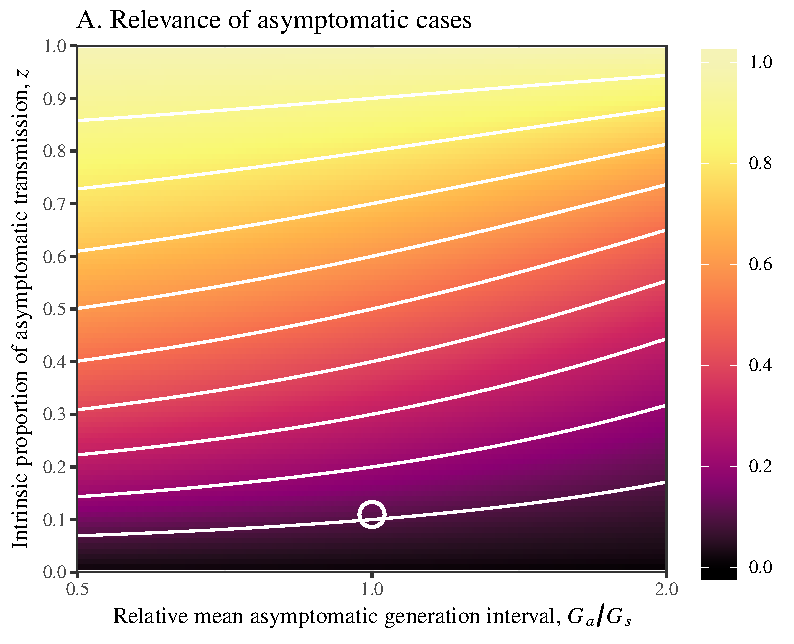
\includegraphics[width=0.4\textwidth]{figheatmap.pdf}
\mbox{\hspace{0.05\textwidth}}
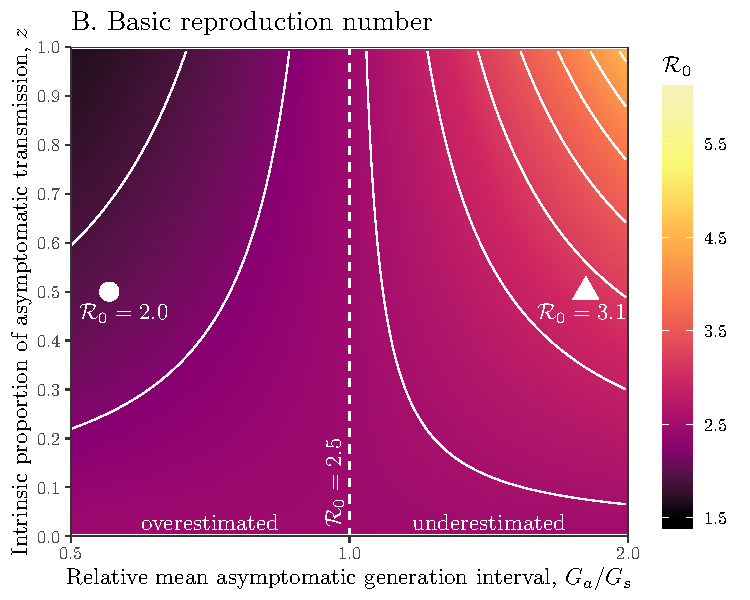
\includegraphics[width=0.4\textwidth]{figheatmap_R0.pdf}\\
\mbox{}\\
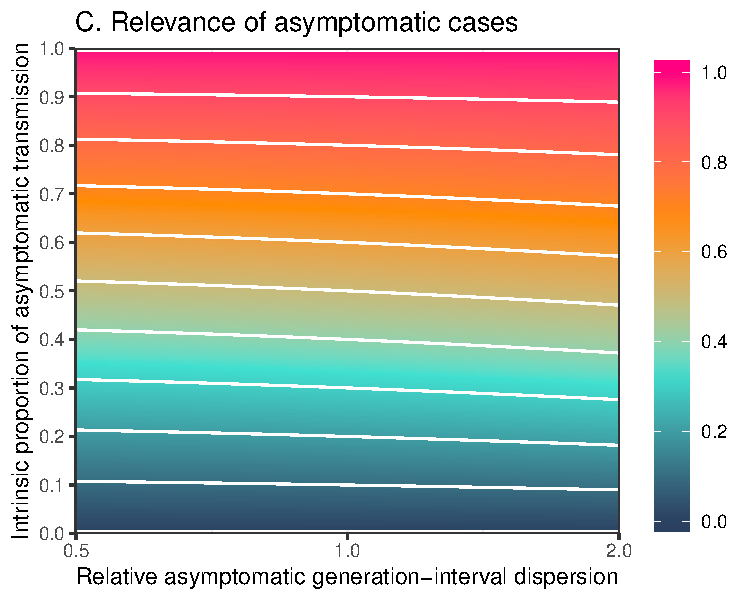
\includegraphics[width=0.4\textwidth]{figheatmap_kappa.pdf}
\mbox{\hspace{0.05\textwidth}}
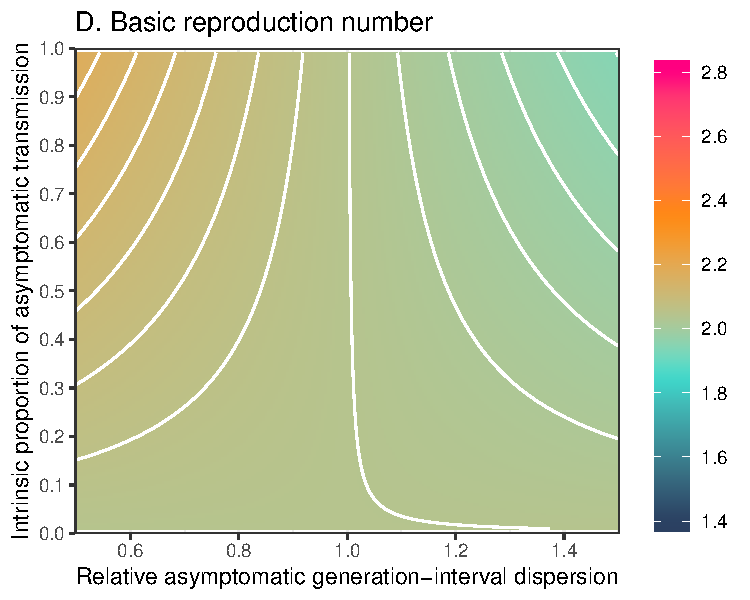
\includegraphics[width=0.4\textwidth]{figheatmap_kappa_R0.pdf}
\caption{Relevance of asymptomatic transmission given variation in
probability that a given, newly infected individual is asymptomatic. (Top) Long/short generation intervals of asymptomatic cases increase/decrease ${\cal{R}}_0$ with decreasing/increasing relevance.
(Bottom) Wide/narrow generation intervals of asymptomatic cases decrease/increase ${\cal{R}}_0$ with increasing/decreasing relevance.
% Technically, renewal equations provide a route to connect
% observed increases in case counts, i.e., ${\cal{R}}_0 = \frac{1}{M(-r)}$
% where $M(-r)=\int_0^{\infty}\mathrm{d} a e^{-ra}g(a)$.
% For the present model,
% $M(r)=qM_E(-r)M_{I_a}(-r)+(1-q)M_E(-r)M_{I_s}(-r)$
% where each of the component functions are $M_E(-r)=\frac{\gamma_e}{\gamma_e+r}$,
% $M_{I_a}(-r)=\frac{\gamma_a}{\gamma_a+r}$, 
% $M_{I_s}(-r)=\frac{\gamma_s}{\gamma_s+r}$,
% and $q$ is the fraction of realized new secondary cases caused by
% asymptomatic individuals.  In all of these heatmaps, $\gamma_e=1/4$,
% $\gamma_s=1/10$, and $r=1/7$. Here, the average duration
% in symptomatic and asymptomatic states are $T_s=1/\gamma_s$ and 
% $T_a=1/\gamma_a$, respectively. Here the filled circle denotes ${\cal{R}}_0\approx 3.12$
% in the event of $p=0$ and $\beta_a=0$, and the open symbols are for $\beta_a/\beta_s=0.5$ and 
% $p=0.5$ and $p=0.9$ for reference.
%Renewal equations provide a route to connect
%observed increases in case counts, i.e.,
%\begin{equation}
%{\cal{R}}_0 = \frac{1}{M(-r)}
%\end{equation}
%where $r$ is the speed of the disease spread and 
%$M(r)$ is related to 
%$g(a)$ (the normalized age of transmission) such that 
%\begin{equation}
%M(r)=\int_0^{\infty}\mathrm{d} a e^{ra}g(a).
%\end{equation}
%For the present model, the moment generating function is
%\begin{equation}
%M(r)=qM_E(r)M_{I_a}(r)+(1-q)M_E(r)M_{I_s}(r)
%\end{equation}
%where each of the component functions are $M_E(-r)=\frac{\gamma_e}{\gamma_e+r}$,
%$M_{I_a}(-r)=\frac{\gamma_a}{\gamma_a+r}$, 
%$M_{I_s}(-r)=\frac{\gamma_s}{\gamma_s+r}$,
%and $q$ is the fraction of realized new secondary cases caused by
%asymptomatic individuals. 
%The relevance $q$ is an unknown feature of
\label{fig.relevance}}
\end{center}
\end{figure*}

 
%We also note that efforts to characterize asymptomatic tranissmion
%should consider its effect on
%the basic reproduction number, which for this SEIR coronavirus-like model is ${\cal{R}}_0=p\left(\frac{\beta_a}{\gamma_a}\right)+ (1-p)\left(\frac{\beta_s}{\gamma_s}\right).$
%%Pooling estimates via a Bayesian approach applied to the early stages of Wuhan case data,
%%suggests ${\cal{R}}_0\approx 3.0$ 
%%with a 95\% confidence interval from 2-4.5.  Yet, that information
%%is not sufficient to disentangle the role of asymptomatic cases, i.e.,
%%what fraction of secondary cases can be ascribed to transmission
%%from asymptomatic cases vs.~symptomatic cases?  
%Strength, ${\cal{R}}_0$ and size $r$
%can be related via a Gamma approximation to the generation
%interval distribution as follows:
%\begin{equation}
%{\cal{R}}^{gamma}=(1+\kappa r \bar{G})^{1/\kappa}
%\end{equation}
%where $\bar{G}$ is the mean generation interval and
%$\kappa$  is the squared coefficient of variation of
%the generation interval.  
%This approximation (explored in Champredon
%et al.) reveals why for a given observed speed,
%increases in the mean generation interval imply
%larger reproduction number. Hence, reports of individuals
%with mild cases that remain infectious for (relatively)
%long periods suggest that the mean generation interval
%could be longer than estimated from symptomatic cases alone - both
%increasing ${\cal{R}}_0$ and driving a larger fraction of secondary cases.
%This inference also reinforces 
%the need to characterize the epidemiological characteristics of asymptomatic transmission.

%than expected. Yet the relevance of asymptomatic cases
%depends on their realized proportion at a population level.

%Renewal equations provide a route to connect
%observed increases in case counts, i.e.,
%\begin{equation}
%{\cal{R}}_0 = \frac{1}{M(-r)}
%\end{equation}
%where $r$ is the speed of the disease spread and $M(r)$ is the
%moment generating function of the generation interval distribution
%$g(a)$ (normalized age of transmission) such that 
%\begin{equation}
%M(r)=\int_0^{\infty}\mathrm{d} a e^{ra}g(a).
%\end{equation}
%For the present model, the moment generating function is
%\begin{equation}
%M(r)=qM_E(r)M_{I_a}(r)+(1-q)M_E(r)M_{I_s}(r)
%\end{equation}
%where each of the component functions are $M_E(-r)=\frac{\gamma_e}{\gamma_e+r}$,
%$M_{I_a}(-r)=\frac{\gamma_a}{\gamma_a+r}$, 
%$M_{I_s}(-r)=\frac{\gamma_s}{\gamma_s+r}$,
%and $q$ is the fraction of realized new secondary cases caused by
%asymptomatic individuals. The relevance $q$ is an unknown feature of
%outbreaks at the population scale, distinct from $p$ the probability of having
%an asymptomatic cases, conditional upon being infected
%but not yet infectious. Hence,
%if one were to observe $r$ (which can vary from country to 
%country and from region to region) then it should be possible
%to link the values $p$ and the relative transmission rates,
%$\beta_a/\beta_s$ to the relevance of asymptomatic transmission
%at the population scale.



%Renewal equations provide a route to connect
%observed increases in case counts, i.e.,
%\begin{equation}
%{\cal{R}}_0 = \frac{1}{M(-r)}
%\end{equation}
%where $r$ is the speed of the disease spread and $M(r)$ is the
%moment generating function of the generation interval distribution
%$g(a)$ (normalized age of transmission) such that 
%\begin{equation}
%M(r)=\int_0^{\infty}\mathrm{d} a e^{ra}g(a).
%\end{equation}
%For the present model, the moment generating function is
%\begin{equation}
%M(r)=qM_E(r)M_{I_a}(r)+(1-q)M_E(r)M_{I_s}(r)
%\end{equation}
%where each of the component functions are $M_E(-r)=\frac{\gamma_e}{\gamma_e+r}$,
%$M_{I_a}(-r)=\frac{\gamma_a}{\gamma_a+r}$, 
%$M_{I_s}(-r)=\frac{\gamma_s}{\gamma_s+r}$,
%and $q$ is the fraction of realized new secondary cases caused by
%asymptomatic individuals. The relevance $q$ is an unknown feature of
%outbreaks at the population scale, distinct from $p$ the probability of having
%an asymptomatic cases, conditional upon being infected
%but not yet infectious. Hence,
%if one were to observe $r$ (which can vary from country to 
%country and from region to region) then it should be possible
%to link the values $p$ and the relative transmission rates,
%$\beta_a/\beta_s$ to the relevance of asymptomatic transmission
%at the population scale.
%
%
%
%
%Hence, recalling the equation for the basic reproduction number
%\begin{equation}
%{\cal{R}}_{0,E}= p\left(\frac{\beta_a}{\gamma_a}\right)+ (1-p)\left(\frac{\beta_s}{\gamma_s}\right)
%\end{equation}
%suggests that 
%This gap between intrinsic and realized transmission routes
%lies at the base of our exploration.
%
%\section{Dynamics}
%We simulate the SEIaIsRD model assuming $N=10^6$ with
%the following initial conditions: $S_0=10^6-1$, $E_0=1$
%and all other elements 0.  The following model vary $p$ from
%0.1 to 0.5 to 0.9.  For various reasons, the parameters are:
%$\gamma_e=1/4$, $\gamma_a=1/42$, $\gamma_s=1/14$,
%$\beta_a=1/14$, $\beta_s=3/14$, $f=0.02$.  The resultant
%value of ${\cal{R}}_0=3$ for all values of $p$, however
%the realized CFR, fraction of asymptomatic cases, and even
%the speed of the disease varies significantly. Hence, we 
%need to adopt a different approach, given that we
%observe a speed, $r$, and yet are uncertain with
%respect to the underlying contribution of asymptomatic
%vs.~symptomatic cases.
%
%\begin{figure*}[h!]
%\begin{center}
%\includegraphics[width=0.9\textwidth]{figseird_base_noname.pdf}\\
%\includegraphics[width=0.9\textwidth]{figseird_base2_noname.pdf}\\
%\includegraphics[width=0.9\textwidth]{figseird_base3_noname.pdf}\\
%\end{center}
%\end{figure*}
%
%\section{Constrained Dynamics}
%Here, we simulate the SEIR model developed
%for coronavirus assuming $N=10^6$ with
%the following initial conditions: $S_0=10^6-1$, $E_0=1$
%and all other elements set to 0.  We assume that the speed of
%the outbreak is $r=1/6$ days$^{-1}$. We further assume that $\gamma_e=1/4$
%(4 days to onset), $\gamma_a=1/42$, $\gamma_s=1/14$, and $p=0.9$.
%How do we solve for the unknown transmission rates, $\beta_a$
%and $\beta_s$?  Alone, it would seem we have a under-determined
%problem, such that
%\begin{equation}
%p\left(\frac{\beta_a}{\gamma_a}\right)+ (1-p)\left(\frac{\beta_s}{\gamma_s}\right)=\frac{1}{M(-r)}.
%\end{equation}
%However, if one assumes that a fraction $q$ of secondary infections are caused by
%asymptomatic individuals, then there is an additional constraint:
%\begin{equation}
%p\frac{\beta_a}{\gamma_a}=\frac{q}{M(-r)}
%\end{equation}
%such that 
%\begin{equation}
%\beta_a = \frac{q\gamma_a}{pM(-r)}.
%\end{equation}
%As a result, then 
%\begin{equation}
%\beta_s = \frac{(1-q)\gamma_s}{(1-p)M(-r)}
%\end{equation}
%In essence, as $q$ varies, then both tranmission rates will have 
%to covary (indeed in a negative fashion) to reconciled the realized
%speed of the outbreak. We now put this into practice for three scenarios,
%all for the case of $p=0.9$ (in which intrinsically most cases
%are asymptomatic):
%\begin{description}
%\item[Short asymptomatic cases] Here we assume
%$\gamma_s=1/14$ (2 week for severe cases) and $\gamma_a=1/2$ 
%(2 day resolution, i.e., a 7-fold change). 
%\item[Long asymptomatic cases] Here we assume
%$\gamma_s=1/14$ (2 week for severe cases) and $\gamma_a=1/42$ 
%(6 week for mild cases)
%\end{description}
%We also assume as before that $f=0.02$ for severe cases. The following 
%results show that we can in fact calculate the correct values of
%$\beta_a$ and $\beta_s$ given variation in $q$.
%It is also important to point out that
%${\cal{R}}_0$ can be extended or decreased with $q$ depending
%on whether $\gamma_a$ is faster or slower relative to $\gamma_s$.
%The key idea there is the same as that for the impact of post-death
%transmission of Ebola virus disease.
%
%For the short duration asymptomatic cases (see Figure~\ref{constrain}), we find the following trade-offs:
%\begin{verbatim}
%         q: [0.0100 0.1000 0.5000 0.9000 0.9900]
%    beta_a: [0.0258 0.2311 0.7857 1.0714 1.1176]
%    beta_s: [3.2898 2.6741 1.0102 0.1531 0.0145]
%        R0: [4.6523 4.1597 2.8286 2.1429 2.0320]
%\end{verbatim}
%whereas for the longer duration asymptomatic cases we find
%\begin{verbatim}
%         q: [0.0100 0.1000 0.5000 0.9000 0.9900]
%    beta_a: [0.0013 0.0132 0.0873 0.2311 0.2843]
%    beta_s: [3.3528 3.2143 2.3571 0.6933 0.0775]
%        R0: [4.7414 5 6.6000 9.7059 10.8553]
%\end{verbatim}
%In the first case, when most illnesses
%are caused by asymptomatic cases, then shorter generation intervals
%for the same growth rate means a lower ${\cal{R}}_0$. Whereas,
%in the second case, when most illnesses are caused by asymptomatic
%cases, then longer generation intervals for the same growth rate
%means a higher ${\cal{R}}_0$.
%\begin{figure*}[b!]
%\begin{center}
%\includegraphics[width=0.9\textwidth]{figconstrain_short_noname.pdf}\\
%\includegraphics[width=0.9\textwidth]{figconstrain_long_noname.pdf}\\
%\caption{Short, mild asymptomatic cases (top) vs. longer, mild asymptomatic
%cases (bottom). For both, common parameters are $\gamma_e=0.25$,
%$\gamma_s=1/14$, $f=0.02$, $p=0.9$, and $r=1/7$.  For the short
%asymptomatic case scenario, $\gamma_a=1/2$ whereas for the long asymptomatic
%case scenario $\gamma_a=1/42$.
%\label{constrain}}
%\end{center}
%\end{figure*}
%
%Finally, in an effort to try and reconcile this, we point out the following
%synthetic figure of outbreaks all with a growth rate of $r=1/7$ by construction, yet differ in vastly different ways based on 3 facets, the value of $p$ (the instrinsic fraction of asymptomatic cases),
%the value of $1/\gamma_a$ (that sets the average duration of asymptomatic cases), and
%the realized value of $q$ (the fraction of secondary cases caused by asymptomatic cases).  As is
%apparent, all disease take off at the same speed, but have very different peak strengths,
%and also, different decomposition of the relative importance of the asymptomatic component.
%What is notable is that the peak size is more driven by $p$ and $\gamma_a$ than by $q$
%(see Figure~\ref{constrain2}).
%\begin{figure*}[bh!]
%\begin{center}
%\includegraphics[width=0.9\textwidth]{package_overlay_p_T.pdf}
%\caption{Synthesis of dynamical results given variation in 
%the intrinsic generation interval of asymptomatic cases (set by $1/\gamma_a$), frequency ($p$), 
%and importance ($q$).
%For all, common parameters are $\gamma_e=0.25$,
%$\gamma_s=1/14$, $f=0.02$, and $r=1/7$.  For the short
%asymptomatic case scenario, $\gamma_a=1/2$ whereas for the long asymptomatic
%case scenario $\gamma_a=1/42$.
%\label{constrain2}}
%\end{center}
%\end{figure*}
%
%%
%%\section{Simulations}
%%Consider an outbreak whose
%%symptomatic cases is ${\cal{R}}_0\approx 3$, such that
%%$\beta_s/\gamma_s=3$.  We further assume that transition from
%%exposed to either $I_a$ or $I_s$ takes 4 days on average,
%%such that $\eta=1/4$.  The following is an example
%%outbreak, in which $\beta_s=\beta_a=3/7$, $\gamma_a=1/45$,
%%and $f=0.02$ (corresponding to a 2\% case fatality rate
%%for symptomatic cases). As is apparent, there is an exponential
%%increase in cases, such that $r\approx 0.30$ days$^{-1}$.
%%In this case, we expect that in the exponential phase,
%%then $I_a/I_s\approx 13.8$.  This prediction is borne out
%%by simulation as in Figure~\ref{fig.ratio}.
%%\begin{figure*}[h!]
%%\begin{center}
%%\includegraphics[width=0.4\textwidth]{figexample1_noname.pdf}
%%\mbox{\hspace{0.05\textwidth}}
%%\includegraphics[width=0.4\textwidth]{figexample1_ratio_noname.pdf}
%%\caption{Asymptomatic to symptomatic case ratio at 
%%the population scale can exceed the ratio of relative case
%%production at the individual scale, when $\gamma_a\ll \gamma_s$.\label{fig.ratio}}
%%\end{center}
%%\end{figure*}
%%Similalry, in the case that asymmptomatic cases rapidly
%%recover, then we expect the population rate to be less then
%%$z$. In the event that $\gamma_a=1$ (7-fold faster than
%%the the symptomatic removal rate) then $r\approx 0.17$ and
%%the ratio is expected to converge to $\approx 2.7$, as shown in Figure~\ref{fig.ratio2}.
%%\begin{figure*}[h!]
%%\begin{center}
%%\includegraphics[width=0.4\textwidth]{figexample2_noname.pdf}
%%\mbox{\hspace{0.05\textwidth}}
%%\includegraphics[width=0.4\textwidth]{figexample2_ratio_noname.pdf}
%%\caption{Asymptomatic to symptomatic case ratio at 
%%the population scale can exceed the ratio of relative case
%%production at the individual scale, when $\gamma_a\gg \gamma_s$.
%%\label{fig.ratio2}
%%}
%%\end{center}
%%\end{figure*}
%%Finally, in the case that asymptomatic cases and symptomatic
%%cases have the same exepcted rudation
%%then we expect the population ratio to be less then
%%$z$. In the event that $\gamma_a=1$ (7-fold faster than
%%the the symptomatic removal rate) then $r\approx 0.26$ and
%%the ratio is expected to converge to $\approx 10$, as shown in Figure~\ref{fig.ratio3}.
%%\begin{figure*}[h!]
%%\begin{center}
%%\includegraphics[width=0.4\textwidth]{figexample3_noname.pdf}
%%\mbox{\hspace{0.05\textwidth}}
%%\includegraphics[width=0.4\textwidth]{figexample3_ratio_noname.pdf}
%%\caption{Asymptomatic to symptomatic case ratio at 
%%the population scale can exceed the ratio of relative case
%%production at the individual scale, when $\gamma_s=\gamma_a$.
%%\label{fig.ratio3}
%%}
%%\end{center}
%%\end{figure*}
%%
%%\section{Stability of the infection-free equilibrium}
%%Consider the following infection subystem, assume $S\approx 1$
%%\begin{eqnarray}
%%\dot{E}&=&\beta_a I_a +\beta_s I_s -\eta E\\
%%\dot{I}_a&=&\frac{z}{z+1}\eta E-\gamma_a I_a\\
%%\dot{I}_s&=&\frac{1}{z+1}\eta E-\gamma_s I_s
%%\end{eqnarray}
%%such that the Jacobian is:
%%\begin{equation}
%%J = \left[
%%\begin{array}{ccc}
%%-\eta & \beta_a & \beta_s \\
%%\frac{z}{z+1}E & -\gamma_a & 0 \\
%%\frac{1}{z+1}E & -\gamma_s & 0 
%%\end{array}
%%\right]
%%\end{equation}
